% Chapter 1

\chapter{Kitaev Quantum Double Model} % Main chapter title

\label{Chapter2} % For referencing the chapter elsewhere, use \ref{Chapter1} 

\lhead{Chapter 2. \emph{Quantum Doubles}} % This is for the header on each page - perhaps a shortened title

%----------------------------------------------------------------------------------------

\section{Introduction to Quantum Double Models}

    This section is heavily inspired by \citep{Reference1}. Given a group $G$, consider a lattice with each edge being associated with a Hilbert space and indexed 
by a group element. A site in the lattice is given by a pair of adjacent vertex and face. For a given site (vertex $v$ and face $f$), define the vertex operator $A^{g}_{v}$ 
and face operator $B^{h}_{s}$ as in figure \ref{fig:A_v_B_p operators} :
\begin{figure}
\centering
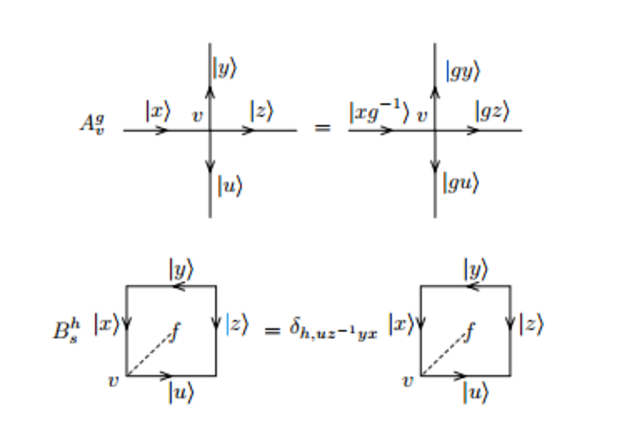
\includegraphics[width=10cm]{A_v_B_p.pdf}
\caption[Definition of Vertex, Face operators]{Definition of the $A_{v}^{g}$ and $B_{s}^{h}$ operators on a arbitrary vertex and face}
\centering
\label{fig:A_v_B_p operators}
\end{figure}

. The Hamiltonain for the lattice is given by 
\begin{center}
  $H = -\varSigma_{v} A_{v} - \varSigma_{f} B_{f}$
\end{center}

\subsection{Ribbon operators, Excitations, Anyon types}
    A ribbion $\xi$ in the lattice is a sequence of adjacent sites connecting two sites $s_{0}$ and $s_{1}$.
The ribbon operator $F^{h,g}_{\xi}$ is defined as in figure \ref{fig:ribbon} : \\
\begin{figure}
\centering
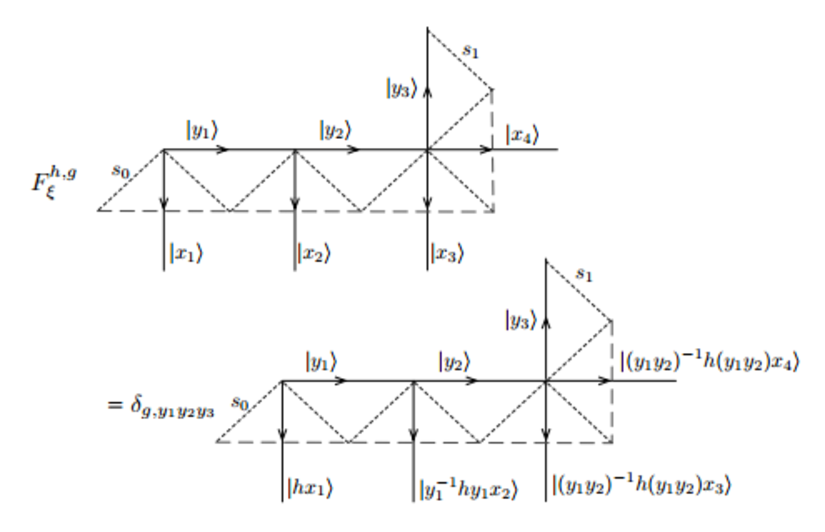
\includegraphics[width=10cm]{Ribbon_operator.pdf}
\caption[Definition of Ribbon operator]{Definition of a ribbon operator on a arbitrary lattice}
\centering
\label{fig:ribbon}
\end{figure}

For a ribbon connecting the sites $s_{0}$ and $s_{1}$, and if any site in the adjacent sequence is given by $t$,
the ribbon operator defined above satisfy the following commutation relationships,
\begin{center}
      [$F^{h,g}_{\xi}$, $A^{k}_{t}$] = [$F^{h,g}_{\xi}$, $B^{s}_{t}$] = 0, \\ 
      $A^{k}_{s_{0}}$ $F^{h,g}_{\xi}$ = $F^{khk^{-1},kg}_{\xi}$ $A^{k}_{s_{0}}$ \\
      $B^{k}_{s_{0}}$ $F^{h,g}_{\xi}$ = $F^{h,g}_{\xi}$ $B^{kh}_{s_{0}}$ \\
      $A^{k}_{s_{1}}$ $F^{h,g}_{\xi}$ = $F^{h,gk^{-1}}_{\xi}$ $A^{k}_{s_{1}}$ \\
      $B^{k}_{s_{1}}$ $F^{h,g}_{\xi}$ = $F^{h,g}_{\xi}$ $B^{g^{-1}h^{-1}gk}_{s_{1}}$
\end{center}

The application of ribbon operator on the ground state, gives rise to quasi-particle excitations at the end of the ribbon. The excitations are independent 
of the topology of the ribbon operator. Therefore the excitations can be moved around the lattice by extending/contracting the ribbon. Fusion of two quasi-particle
excitations can be achieved by moving them to the same site and fusing them, the resultant describes a system of anyons.

Anyon types for a Kitaev Quantum Double are in one-to-one correspondance with the irreducdible representations of the Drinfeld Double of the group, which are in 
one-to-one correspondace with the irreducible representations of the centralizers of the conjugacy classes of the group \citep{Reference1}. The method to compute this for any finite
group has been presented in Appendix \ref{AppendixA} and has been computed for various groups like $Z_{2}, S_{3}, D_{4}$ the first one being the case of Toric Code.

%----------------------------------------------------------------------------------------

\subsection{Introduction of boundaries, Condensates, Ribbon operators}

	Consider a lattice as above but with a boundary, that is with a lattice on one half and nothing on the other side, and the edges connecting both the half planes being
the boundary. The edges on the boundary are associated with a Hilbert space $C[K]$, where $C$ is the complex field and $K$ $\subset$ $G$ and indexed by elements of $K$. The 
vertex and the face operator for the internal lattice remain as defined in the introduction, but for the boundary the vertex and face operators are defined as follows :
\begin{center}
 $A^{K}_{s} = \frac{1}{|K|} \varSigma_{k \in K} A^{k}_{s}$ \\
 $B^{K}_{s} = \varSigma_{k \in K} B^{k}_{s}$
\end{center}
where $s$ is a site on the boundary.

The hamiltonian of the system with the boundary is given by,
\begin{center}
 $H = -\varSigma_{v} A_{v} - \varSigma_{f} B_{f} - \varSigma_{s} (A^{K}_{s} + B^{K}_{s})$
\end{center}

      To construct a ribbon $T = \varSigma_{h,g}c_{h,g}F^{h,g}_{\xi}$, connecting the sites in the bulk to the sites on the boundary, the ribbon should satisfy the commutation relationship mentioned in the 
previous section
\begin{center}
      $A^{k}_{s_{0}}$ $T$ = $T$ $A^{k}_{s_{0}}$ \\
      $B^{k}_{s_{0}}$ $T$ = $F^{h,g}_{\xi}$ $B^{kh}_{s_{0}}$ \\
\end{center}

along with the following commutation relationships :
\begin{center}
        $[T, A^{K}_{s_{0}}] = 0$ , \\
        $[T, B^{K}_{s_{0}}] = 0$
\end{center}

Solving for $T$, gives 
\begin{center}
    $T^{(k,g)} = \varSigma_{l \in K} F^{(lkl^{-1},lg^{-1})}_{\xi}$ 
\end{center}

We now present the various $T^{(k,g)}$ for the subgroups of $S_{3}$. Consider the subgroup 
$K$ = $G$, we compute the $T^{(k,g)}$ for various combinations of $k$ and $g$.

\subsubsection{Ribbon operators in a lattice with boundaries in the case of $S_{3}$}
Using the following snippet, we group the summation for each of the subgroup 
\begin{lstlisting}[frame=single]
sage: G =  SymmetricGroup(3)
sage: K = G.subgroups()[5]
sage: x = []
sage: y = []
sage: for k in K:
    for g in G:
        for l in K:
            x.append([l*k*l^-1, l*g^-1])
....: 
sage: for i in range(len(x)/6):
    y.append(x[6*i:6*(i+1)])

sage: y
# The first element is given by lkl^-1 and second element by lg^-1, which allows
# us to read  of the T^{(k,g)} from the first element of every summation. 

# For the case k = e and g running over all group elements.

[[[(), ()], [(), (2,3)], [(), (1,2,3)], [(), (1,2)], 
[(), (1,3,2)], [(), (1,3)]],
[[(), (1,2)], [(), (1,2,3)], [(), (2,3)], [(), ()], 
[(), (1,3)], [(), (1,3,2)]],
[[(), (1,3,2)], [(), (1,3)], [(), ()], [(), (2,3)], 
[(), (1,2,3)], [(), (1,2)]],
[[(), (1,2,3)], [(), (1,2)], [(), (1,3,2)], [(), (1,3)], 
[(), ()], [(), (2,3)]],
[[(), (2,3)], [(), ()], [(), (1,3)], [(), (1,3,2)], 
[(), (1,2)], [(), (1,2,3)]],
[[(), (1,3)], [(), (1,3,2)], [(), (1,2)], [(), (1,2,3)], 
[(), (2,3)], [(), ()]],

# Therefore, T^{(e,e)} is given by the first sum and similarly others. 
# So for the element e, the operators collapse to a single operator given by 
# T^{(e,g)} = summation(F^{(e,g)}) over all g \in G. Implying all the six collapse to a single operator.

# For the case k = (2,3) and g running over all group elements.

[[(2,3), ()], [(2,3), (2,3)], [(1,2), (1,2,3)], [(1,3), (1,2)], 
[(1,3), (1,3,2)], [(1,2), (1,3)]],
[[(2,3), (1,2)], [(2,3), (1,2,3)], [(1,2), (2,3)], [(1,3), ()], 
[(1,3), (1,3)], [(1,2), (1,3,2)]],
[[(2,3), (1,3,2)], [(2,3), (1,3)], [(1,2), ()], [(1,3), (2,3)], 
[(1,3), (1,2,3)], [(1,2), (1,2)]],
[[(2,3), (1,2,3)], [(2,3), (1,2)], [(1,2), (1,3,2)], [(1,3), (1,3)], 
[(1,3), ()], [(1,2), (2,3)]],
[[(2,3), (2,3)], [(2,3), ()], [(1,2), (1,3)], [(1,3), (1,3,2)],
[(1,3), (1,2)], [(1,2), (1,2,3)]],
[[(2,3), (1,3)], [(2,3), (1,3,2)], [(1,2), (1,2)], [(1,3), (1,2,3)],
[(1,3), (2,3)], [(1,2), ()]],
  
# In this case, (Performing a right multiplication gives the same results !)
# T^{((2,3), e)} = T^{((2,3), (2,3))}, 
# T^{((2,3), (1,2))} = T^{((2,3), (1,3,2))} 
# T^{((2,3), (1,2,3))} = T^{((2,3), (1,3))} 

# Therefore 6 operators reduce to 3.

# For the case k = (1,2,3) and g running over all group elements.

[[(1,2,3), ()], [(1,3,2), (2,3)], [(1,2,3), (1,2,3)], [(1,3,2), (1,2)],
[(1,2,3), (1,3,2)], [(1,3,2), (1,3)]],
[[(1,2,3), (1,2)], [(1,3,2), (1,2,3)], [(1,2,3), (2,3)], [(1,3,2), ()],
[(1,2,3), (1,3)], [(1,3,2), (1,3,2)]],
[[(1,2,3), (1,3,2)], [(1,3,2), (1,3)], [(1,2,3), ()], [(1,3,2), (2,3)],
[(1,2,3), (1,2,3)], [(1,3,2), (1,2)]],
[[(1,2,3), (1,2,3)], [(1,3,2), (1,2)], [(1,2,3), (1,3,2)], [(1,3,2), (1,3)],
[(1,2,3), ()], [(1,3,2), (2,3)]],
[[(1,2,3), (2,3)], [(1,3,2), ()], [(1,2,3), (1,3)], [(1,3,2), (1,3,2)],
[(1,2,3), (1,2)], [(1,3,2), (1,2,3)]],
[[(1,2,3), (1,3)], [(1,3,2), (1,3,2)], [(1,2,3), (1,2)], [(1,3,2), (1,2,3)],
[(1,2,3), (2,3)], [(1,3,2), ()]],

# In this case, again using the same rule as above it is easy to see
# T^{((1,2,3), e)} = T^{((1,2,3), (1,2,3))} = T^{((1,2,3), (1,3,2))}
# T^{((1,2,3), (1,2))} = T^{((1,2,3), (1,3))} = T^{((1,2,3), (2,3))}
  
# Therefore 6 operators collapse to 2.  

# For the case k = (1,2) and g running over all group elements.

[[(1,2), ()], [(1,3), (2,3)], [(1,3), (1,2,3)], [(1,2), (1,2)],
[(2,3), (1,3,2)], [(2,3), (1,3)]],
[[(1,2), (1,2)], [(1,3), (1,2,3)], [(1,3), (2,3)], [(1,2), ()],
[(2,3), (1,3)], [(2,3), (1,3,2)]],
[[(1,2), (1,3,2)], [(1,3), (1,3)], [(1,3), ()], [(1,2), (2,3)],
[(2,3), (1,2,3)], [(2,3), (1,2)]],
[[(1,2), (1,2,3)], [(1,3), (1,2)], [(1,3), (1,3,2)], [(1,2), (1,3)],
[(2,3), ()], [(2,3), (2,3)]],
[[(1,2), (2,3)], [(1,3), ()], [(1,3), (1,3)], [(1,2), (1,3,2)],
[(2,3), (1,2)], [(2,3), (1,2,3)]],
[[(1,2), (1,3)], [(1,3), (1,3,2)], [(1,3), (1,2)], [(1,2), (1,2,3)],
[(2,3), (2,3)], [(2,3), ()]]

# In this case, again using the same rule as above it is easy to see
# T^{((1,2), e)} = T^{((1,2), (1,2))}, 
# T^{((1,2), (1,3))} = T^{((1,2), (1,3,2))} 
# T^{((1,2), (1,2,3))} = T^{((1,2), (2,3))} 

# But in this case we also have 
# T^{((1,2), e)} = T^{((2,3), (1,2,3))}
# T^{((1,2), (1,3))} = T^{((2,3), e)}
# T^{((1,2), (1,2,3))} = T^{((2,3), (1,3,2))

# So again in this case 6  operators reduce to 3 but these are  mapped to the previous maps.

# For the case k = (1,3,2) and g running over all group elements.

[[(1,3,2), ()], [(1,2,3), (2,3)], [(1,3,2), (1,2,3)], [(1,2,3), (1,2)],
[(1,3,2), (1,3,2)], [(1,2,3), (1,3)]],
[[(1,3,2), (1,2)], [(1,2,3), (1,2,3)], [(1,3,2), (2,3)], [(1,2,3), ()],
[(1,3,2), (1,3)], [(1,2,3), (1,3,2)]],
[[(1,3,2), (1,3,2)], [(1,2,3), (1,3)], [(1,3,2), ()], [(1,2,3), (2,3)],
[(1,3,2), (1,2,3)], [(1,2,3), (1,2)]],
[[(1,3,2), (1,2,3)], [(1,2,3), (1,2)], [(1,3,2), (1,3,2)], [(1,2,3), (1,3)],
[(1,3,2), ()], [(1,2,3), (2,3)]],
[[(1,3,2), (2,3)], [(1,2,3), ()], [(1,3,2), (1,3)], [(1,2,3), (1,3,2)],
[(1,3,2), (1,2)], [(1,2,3), (1,2,3)]],
[[(1,3,2), (1,3)], [(1,2,3), (1,3,2)], [(1,3,2), (1,2)], [(1,2,3), (1,2,3)],
[(1,3,2), (2,3)], [(1,2,3), ()]],

# In this case, again using the same rule as above it is easy to see
# T^{((1,3,2), e)} = T^{((1,3,2), (1,3,2))} = T^{((1,3,2), (1,2,3))}
# T^{((1,2,3), (1,2))} = T^{((1,2,3), (1,3))} = T^{((1,2,3), (2,3))}

# But in this case we also have 
# T^{((1,3,2), e)} = T^{((1,2,3), (1,2))}
# T^{((1,3,2), (1,2))} = T^{((1,2,3), e)}

# As expected we have a reduction from 6 to 2, but these are  again mapped.

# For the case k = (1,2) and g running over all group elements.
[[(1,3), ()], [(1,2), (2,3)], [(2,3), (1,2,3)], [(2,3), (1,2)],
[(1,2), (1,3,2)], [(1,3), (1,3)]],
[[(1,3), (1,2)], [(1,2), (1,2,3)], [(2,3), (2,3)], [(2,3), ()],
[(1,2), (1,3)], [(1,3), (1,3,2)]],
[[(1,3), (1,3,2)], [(1,2), (1,3)], [(2,3), ()], [(2,3), (2,3)],
[(1,2), (1,2,3)], [(1,3), (1,2)]],
[[(1,3), (1,2,3)], [(1,2), (1,2)], [(2,3), (1,3,2)], [(2,3), (1,3)],
[(1,2), ()], [(1,3), (2,3)]],
[[(1,3), (2,3)], [(1,2), ()], [(2,3), (1,3)], [(2,3), (1,3,2)],
[(1,2), (1,2)], [(1,3), (1,2,3)]],
[[(1,3), (1,3)], [(1,2), (1,3,2)], [(2,3), (1,2)], [(2,3), (1,2,3)],
[(1,2), (2,3)], [(1,3), ()]]]

# In this case, again using the same rule as above it is easy to see
# T^{((1,3), e)} = T^{((1,3), (1,3))}, 
# T^{((1,3), (1,2,3))} = T^{((1,3), (1,2))} 
# T^{((1,3), (1,3,2))} = T^{((1,3), (2,3))} 

# But in this case we also have 
# T^{((1,3), e)} = T^{((1,2), (2,3))}
# T^{((1,3), (1,2,3))} = T^{((1,2), (1,3,2)}
# T^{((1,3), (1,3,2))} = T^{((1,2), (1,2))

# So again in this case 6  operators reduce to 3 but these are  mapped to the previous maps.

\end{lstlisting}

So in the above case where $K$ = $G$ we have reduced 36 operators to 6 unique operators.

Carrying out a similar analysis for $K$ = $\{e\}$, we again end up with 6 operators as follows :

\begin{lstlisting}[frame=single]
sage: G = SymmetricGroup(3)
sage: K = G.subgroups()[0]
sage: K
Subgroup of (Symmetric group of order 3! as a permutation group) generated by [()]
sage: for k in K:
    for g in G:
        for l in K:
            print k,g,l*k*l^-1, l*g^-1
....: 
() () () ()
() (1,2) () (1,2)
() (1,2,3) () (1,3,2)
() (1,3,2) () (1,2,3)
() (2,3) () (2,3)
() (1,3) () (1,3)
\end{lstlisting}

Hence the unique 6 operators are given by $T^{(e,e)}$, $T^{(e,(1,2))}$, $T^{(e,(2,3))}$, $T^{(e,(1,3))}$, $T^{(e,(1,2,3))}$, $T^{(e,(1,3,2))}$ give
out $F^{(e,e)}$, $F^{(e,(1,2))}$, $F^{(e,(2,3))}$, $F^{(e,(1,3))}$, $F^{(e,(1,2,3))}$, $F^{(e,(1,3,2))}$ in terms of $F_{\xi}^{(h,g)}$ which is defined on the sites.

Carrying out a similar analysis for $K$ = $\{e, \tau\}$, we again end up with 6 operators as follows :

\begin{lstlisting}[frame=single]
sage: G = SymmetricGroup(3)
sage: K = G.subgroups()[1]
sage: K
Subgroup of (Symmetric group of order 3! as a permutation group) generated by [(2,3)]
sage: for k in K:
    for g in G:
        for l in K:
            print k,g,l*k*l^-1, l*g^-1
() () () ()
() () () (2,3)
() (1,2) () (1,2)
() (1,2) () (1,2,3)
() (1,2,3) () (1,3,2)
() (1,2,3) () (1,3)
() (1,3,2) () (1,2,3)
() (1,3,2) () (1,2)
() (2,3) () (2,3)
() (2,3) () ()
() (1,3) () (1,3)
() (1,3) () (1,3,2)
(2,3) () (2,3) ()
(2,3) () (2,3) (2,3)
(2,3) (1,2) (2,3) (1,2)
(2,3) (1,2) (2,3) (1,2,3)
(2,3) (1,2,3) (2,3) (1,3,2)
(2,3) (1,2,3) (2,3) (1,3)
(2,3) (1,3,2) (2,3) (1,2,3)
(2,3) (1,3,2) (2,3) (1,2)
(2,3) (2,3) (2,3) (2,3)
(2,3) (2,3) (2,3) ()
(2,3) (1,3) (2,3) (1,3)
(2,3) (1,3) (2,3) (1,3,2) 
\end{lstlisting}

It is easy to see that the 12 operators reduce to unique 6, \\
$T^{(e,e)}$ = $F^{(e,e)}$ + $F^{(e,(2,3))}$, \\
$T^{(e,(1,2))}$ = $F^{(e,(1,2))}$ + $F^{(e,(1,2,3))}$, \\ 
$T^{(e,(1,2,3))}$ = $F^{(e,1,3,2)}$ + $F^{(e,(1,3))}$, \\
$T^{((2,3),e)}$ = $F^{((2,3),e)}$ + $F^{((2,3),(2,3))}$,\\
$T^{((2,3),(1,2))}$ = $F^{((2,3),(1,2))}$ + $F^{((2,3),(1,2,3))}$,\\
$T^{((2,3),(1,2,3)}$ = $F^{((2,3),(1,3,2))}$ + $F^{((2,3),(1,3))}$,\\

\subsubsection{Explicit Ribbon operators with boundary $K = \{e, \tau\} \subset S_{3}$ in terms of basis}
The section aims to present the explicit form of the operators generated in the case of $K$ = $\{e, \tau\}$,
in terms of the basis of the algebra of the ribbon operators \citep{Reference2}. The $F$ operators are represented 
in terms of the basis $F^{RC}u(i,j)v(i',j')$, where $R$ is the irreducible representation of the 
center of the conjugacy class $C$, is given by:
\begin{center}
$F_{\xi}^{h,g}$ = $\Sigma_{R \in {N_{C}}_{irred}} \Sigma_{j,j'=1}^{n_{R}} \Gamma^{j,j'}_{R}(n_{(h,g)})F^{RC}u(i,j)v(i',j')$ 
\end{center}
where $h^{-1} \in C$, $n_{(h,g)}$ = $q_{i(h^{-1})}^{-1}gq_{i(g^{-1}h^{-1}g)}$  Here $\Gamma$ is the unitary matrix representation of the element $n_{(h,g)}$. We list the representation of $S_3$ as it 
is the center of the conjugacy class of $e$.

\begin{tabular}{| l | l | l | l |}
 \hline 
 Elements  & 1-dim & 1-dim & 2-dim \\
 $e$       &  [1] & [1] &  $\begin{bmatrix}
			    1 & 0 \\
			    0 & 1 \\
			    \end{bmatrix}$ \\
 $(1,2,3)$ &  [1] & [1] & $\begin{bmatrix}
			    -\frac{1}{2} & \frac{\sqrt{3}}{2} \\
			    -\frac{\sqrt{3}}{2} & -\frac{1}{2} \\
			    \end{bmatrix}$ \\
 $(1,3,2)$ &  [1] & [1] & $\begin{bmatrix}
			    -\frac{1}{2} & -\frac{\sqrt{3}}{2} \\
			     \frac{\sqrt{3}}{2} & -\frac{1}{2} \\
			    \end{bmatrix}$ \\
 $(1,2)$   &  [1] & [-1] & $\begin{bmatrix}
			    -1 & 0 \\
			     0 & 1  \\
			    \end{bmatrix}$ \\
 $(2,3)$   &  [1] & [-1] & $\begin{bmatrix}
			    \frac{1}{2} & \frac{\sqrt{3}}{2} \\
			    \frac{\sqrt{3}}{2} & -\frac{1}{2} \\
			    \end{bmatrix}$ \\
 $(1,3)$   &  [1] & [-1] &  $\begin{bmatrix}
			    \frac{1}{2} & -\frac{\sqrt{3}}{2} \\
			    -\frac{\sqrt{3}}{2} & -\frac{1}{2} \\
			    \end{bmatrix}$\\
 \hline
\end{tabular}

$F^{(e,e)}$, here $h^{-1}$ is in the conjugacy class of $e$ and its centralizer is $S_{3}$ itself. So we have three irreps $\pi_{1}, \pi_{2}, \pi_{3}$ whose degrees are 1,1,2. Therefore $F^{(e,e)}$ 
is given by :
\begin{center}
$\Gamma^{1,1}_{\pi_{1}}(n_{(e,e)})F^{\pi_{1}\bar{e}}u(i,1)v(i',1) + \Gamma^{1,1}_{\pi_{2}}(n_{(e,e)})F^{\pi_{2}\bar{e}}u(i,1)v(i',1) 
              + \Gamma^{1,1}_{\pi_{3}}(n_{(e,e)})F^{\pi_{3}\bar{e}}u(i,1)v(i',1) + \Gamma^{1,2}_{\pi_{3}}(n_{(e,e)})F^{\pi_{3}\bar{e}}u(i,1)v(i',2)
              + \Gamma^{2,1}_{\pi_{3}}(n_{(e,e)})F^{\pi_{3}\bar{e}}u(2,1)v(i',1) + \Gamma^{2,2}_{\pi_{3}}(n_{(e,e)})F^{\pi_{3}\bar{e}}u(i,2)v(i',2)$
\end{center}
which reduces to 
\begin{center}
$F^{(e,e)}$ = $F^{\pi_{1}\bar{e}}u(i,1)v(i',1) + F^{\pi_{2}\bar{e}}u(i,1)v(i',1) 
              + F^{\pi_{3}\bar{e}}u(i,1)v(i',1) + F^{\pi_{3}\bar{e}}u(i,2)v(i',2)$
\end{center}

$F^{(e,(2,3))}$ is given by a similar structure, noting that $n_{(e,(2,3))} = (2,3)$, therefore the sum reduces to
\begin{center}
$F^{(e,(2,3))}$ = $F^{\pi_{1}\bar{e}}u(i,1)v(i',1) - F^{\pi_{2}\bar{e}}u(i,1)v(i',1) 
              + \frac{1}{2}F^{\pi_{3}\bar{e}}u(i,1)v(i',1) + \frac{\sqrt{3}}{2}F^{\pi_{3}\bar{e}}u(i,1)v(i',2)
              + \frac{\sqrt{3}}{2}F^{\pi_{3}\bar{e}}u(i,2)v(i',1) - \frac{1}{2}F^{\pi_{3}\bar{e}}u(i,2)v(i',2)$
\end{center}

Therefore  $T^{(e,e)}$ = $F^{(e,e)}$ + $F^{(e,(2,3))}$, is given by \\
\begin{center}
$T^{(e,e)}$ = $2F^{\pi_{1}\bar{e}}u(i,1)v(i',1) + \frac{3}{2}F^{\pi_{3}\bar{e}}u(i,1)v(i',1) 
                    + \frac{\sqrt{3}}{2}F^{\pi_{3}\bar{e}}u(i,1)v(i',2) + \frac{\sqrt{3}}{2}F^{\pi_{3}\bar{e}}u(i,2)v(i',1) 
                    + \frac{1}{2}F^{\pi_{3}\bar{e}}u(i,2)v(i',2)$
\end{center}

On similar lines, $T^{(e,(1,2))}$ = $F^{(e,(1,2))}$ + $F^{(e,(1,2,3))}$ we need to compute $F^{(e,(1,2))}$ and $F^{(e,(1,2,3))}$

For $F^{(e,(1,2))}$, we need $n_{(e,(1,2))} = (1,2)$ and hence 
\begin{center}
$F^{(e,(1,2))}$ = $F^{\pi_{1}\bar{e}}u(i,1)v(i',1) - F^{\pi_{2}\bar{e}}u(i,1)v(i',1) 
              - F^{\pi_{3}\bar{e}}u(i,1)v(i',1) + F^{\pi_{3}\bar{e}}u(i,2)v(i',2)$
\end{center}
For $F^{(e,(1,2,3))}$, we need $n_{(e,(1,2,3))} = (1,2,3)$ and hence
\begin{center}
$F^{(e,(1,2,3))}$ = $F^{\pi_{1}\bar{e}}u(i,1)v(i',1) + F^{\pi_{2}\bar{e}}u(i,1)v(i',1) 
              - \frac{1}{2}F^{\pi_{3}\bar{e}}u(i,1)v(i',1) + \frac{\sqrt{3}}{2}F^{\pi_{3}\bar{e}}u(i,1)v(i',2)
              - \frac{\sqrt{3}}{2}F^{\pi_{3}\bar{e}}u(i,2)v(i',1) - \frac{1}{2}F^{\pi_{3}\bar{e}}u(i,2)v(i',2)$
\end{center}

Therefore $T^{(e,(1,2))}$ is given by 
\begin{center}
$T^{(e,(1,2))}$ = $2F^{\pi_{1}\bar{e}}u(i,1)v(i',1) - \frac{3}{2}F^{\pi_{3}\bar{e}}u(i,1)v(i',1) 
                    + \frac{\sqrt{3}}{2}F^{\pi_{3}\bar{e}}u(i,1)v(i',2) - \frac{\sqrt{3}}{2}F^{\pi_{3}\bar{e}}u(i,2)v(i',1) 
                    + \frac{1}{2}F^{\pi_{3}\bar{e}}u(i,2)v(i',2)$
\end{center}

On similar lines, $T^{(e,(1,2,3))}$ = $F^{(e,(1,3,2))}$ + $F^{(e,(1,3))}$ we need to compute $F^{(e,(1,3,2))}$ and $F^{(e,(1,3))}$

For $F^{(e,(1,3,2))}$, we need $n_{(e,(1,3,2))} = (1,3,2)$ and hence 
\begin{center}
$F^{(e,(1,3,2))}$ = $F^{\pi_{1}\bar{e}}u(i,1)v(i',1) + F^{\pi_{2}\bar{e}}u(i,1)v(i',1) 
              - \frac{1}{2}F^{\pi_{3}\bar{e}}u(i,1)v(i',1) - \frac{\sqrt{3}}{2}F^{\pi_{3}\bar{e}}u(i,1)v(i',2)
              + \frac{\sqrt{3}}{2}F^{\pi_{3}\bar{e}}u(i,2)v(i',1) - \frac{1}{2}F^{\pi_{3}\bar{e}}u(i,2)v(i',2)$
\end{center}
For $F^{(e,(1,3))}$, we need $n_{(e,(1,3))} = (1,3)$ and hence
\begin{center}
$F^{(e,(1,3))}$ = $F^{\pi_{1}\bar{e}}u(i,1)v(i',1) - F^{\pi_{2}\bar{e}}u(i,1)v(i',1) 
              + \frac{1}{2}F^{\pi_{3}\bar{e}}u(i,1)v(i',1) - \frac{\sqrt{3}}{2}F^{\pi_{3}\bar{e}}u(i,1)v(i',2)
              - \frac{\sqrt{3}}{2}F^{\pi_{3}\bar{e}}u(i,2)v(i',1) - \frac{1}{2}F^{\pi_{3}\bar{e}}u(i,2)v(i',2)$
\end{center}

Therefore $T^{(e,(1,3,2))}$ is given by 
\begin{center}
$T^{(e,(1,3,2))}$ = $2F^{\pi_{1}\bar{e}}u(i,1)v(i',1) - \sqrt{3}F^{\pi_{3}\bar{e}}u(i,1)v(i',2) 
                    -F^{\pi_{3}\bar{e}}u(i,2)v(i',2)$
\end{center}


% $T^{((2,3),e)}$ = $F^{((2,3),e)}$ + $F^{((2,3),(2,3))}$,\\
% $T^{((2,3),(1,2))}$ = $F^{((2,3),(1,2))}$ + $F^{((2,3),(1,2,3))}$,\\
% $T^{((2,3),(1,2,3)}$ = $F^{((2,3),(1,3,2))}$ + $F^{((2,3),(1,3))}$,\\

On similar lines, $T^{((2,3),e)}$ = $F^{((2,3),e)}$ + $F^{((2,3),(2,3))}$ we need to compute $F^{((2,3),e)}$ and $F^{((2,3),(2,3))}$

For $F^{((2,3),e)}$, we need $n_{((2,3),e)} = e$ and hence 
\begin{center}
$F^{((2,3),e)}$ = $F^{\pi_{1}\bar{\tau}}u(i,1)v(i',1) + F^{\pi_{2}\bar{\tau}}u(i,1)v(i',1)$
\end{center}

For $F^{((2,3),(2,3))}$, we need $n_{((2,3),(2,3))} = (2,3)$ and hence
\begin{center}
$F^{(2,3),e}$ = $F^{\pi_{1}\bar{\tau}}u(i,1)v(i',1) - F^{\pi_{2}\bar{\tau}}u(i,1)v(i',1)$
\end{center}

Therefore $T^{(2,3),e)}$ is given by 
\begin{center}
$T^{((2,3),e)}$ = $2F^{\pi_{1}\bar{\tau}}u(i,1)v(i',1)$ % v lo i' index vary avutundi adi calculation chubettali
\end{center}

Similarly we have the other two ribbon operators given by 

\begin{center}
$T^{((2,3),(1,2))}$ = $2F^{\pi_{1}\bar{\tau}}u(i,1)v(i',1)$ % v lo i' index vary avutundi adi calculation chubettali
\end{center}

\begin{center}
$T^{((2,3),(1,2,3))}$ = $2F^{\pi_{1}\bar{\tau}}u(i,1)v(i',1)$ % v lo i' index vary avutundi adi calculation chubettali
\end{center}

Here the $i'$ varies over 1,2,3, giving rise to different $T$ operators. 

The above representation was computed with an idea to further reduce the number of operators, with an expectation of compressing 6 operators 
to three which further give rise to three ground states (thus verifying the fact that there are three ground states in the given system). 
But, as seen this happens to be a basis transformation, the calculation of the ground state is presented in the next section.

\subsubsection{Excitation condensation on various boundaries for $D(S_{3})$}
           The excitations in a Quantum Double model are given by irreps of the centralizers of the conjugacy class of the group. The character of a particular
representation $\pi$ is given by  $\chi_{(\bar{a}, \pi)}$ : 
\begin{center}
$\chi_{(\bar{a}, \pi)}(gh^{*}) = \delta_{h\in\bar{a}}\delta_{gh, hg} tr_{\pi}(k_{h}^{-1}gk_{h})$, 
\end{center}
as $h\in\bar{a}$ is one of the conditions to be satisfied, $k_{h}$ is some element in $G$ such that $h = k_{h}ak_{h}^{-1}$

For $k \in K$ and $g \in G$ define $|\psi^{k,g}_{K}> = T^{(k,g)} |\psi_{K}>$ and let $A(K)$ be the span of these vectors. Let $\chi_{A(K)}$ be the 
character of the representation $A(K)$. 
\begin{center}
$\chi_{A(K)}(hg^{*}) = \frac{1}{|K|}\delta_{gh,hg}\varSigma_{x \in G}\delta_{xgx^{-1} \in K}\delta_{xhx^{-1} \in K}$
\end{center}

To compute whether a particular excitation condenses at the boundary, the inner product defined as 
\begin{center}
 $<\chi_{1}, \chi_{2}> = \frac{1}{|G|} \varSigma_{g,h}(\chi_{1}(gh^{*})^{*}\chi_{2}(gh^{*})$
\end{center}
of the above characters is observed, if it is positive the excitation associated with the irrep of $D(G)$ condenses at the boundary.

Consider the case of $S_{3}$, the following are the conjugacy classes $\{e\}$, $\{\tau\}$ and $\{\sigma\}$ where $\{e, \tau, \sigma\}$ form the presentation of the group.
The corresponding centralizer for each of the conjugacy classes are given by $S_{3}$, $\{e, \tau\}$, $\{e, \sigma, \sigma^{-1}\}$, whose corresponding irreps are
$\{1$, sign, $\pi\}$, (where $1$, sign are one dimensional irreps of $S_{3}$ and $\pi$ is a two dimensional irrep.),  $\{1, -1\}$, $\{1, \omega, \omega^{*}\}$. For
the case of $S_{3}$ the irreps of $D(S_{3})$ are indexed by $V_{a, \pi}$ where $\pi$ is the representation of the centralizer of the conjugacy class of $a$.
Put together there are eight excitations in $D(S_{3})$ given by $V_{e, \pi_{1}}$, $V_{e, \pi_{2}}$, $V_{e, \pi_{3}}$, $V_{\tau, \pi_{1}}$, $V_{\tau, \pi_{2}}$, 
$V_{\sigma, \pi_{1}}$, $V_{\sigma, \pi_{2}}$, $V_{sigma, \pi_{3}}$ which are labelled and referred by $A, B, C, D, E, F, G, G$.
The following snippet has been used to compute the inner product, 
\begin{lstlisting}[frame=single]
sage: def character_1_irred(G, subgroup, g, h):
    sum = 0
    if h*g == g*h:
        for i in G:
            if i*g*i^-1 in subgroup and i*h*i^-1 in subgroup:
                sum = sum + 1
    return sum/len(subgroup)
....: 
sage: def character_2_irred(G, conjugacy_class, g, h):
    k_h = 0
    for i in G:
        if h*i == i*conjugacy_class.an_element():
            k_h = i
            break
    if g*h == h*g and k_h != 0:
        return  k_h^-1*g*k_h
    else:
        return 0
\end{lstlisting}

In the above snippet the first function returns the irreducible character of $A(K)$. The second function returns the element on which the trace is to be calculated by relating to
the representation of the centralizer of the conjugacy class. 

$S_{3}$ is taken as an example to explain further. First the subgroups and the conjugacy classes of $S_{3}$ are presented. 

\begin{lstlisting}[frame=single]
sage: G = SymmetricGroup(3)
sage: for i in G.subgroups():
....:     print i
....: 
Subgroup of (Symmetric group of order 3! as a permutation group) 
generated by [()]
Subgroup of (Symmetric group of order 3! as a permutation group) 
generated by [(2,3)]
Subgroup of (Symmetric group of order 3! as a permutation group) 
generated by [(1,2)]
Subgroup of (Symmetric group of order 3! as a permutation group) 
generated by [(1,3)]
Subgroup of (Symmetric group of order 3! as a permutation group) 
generated by [(1,2,3)]
Subgroup of (Symmetric group of order 3! as a permutation group) 
generated by [(2,3), (1,2,3)]

sage: for i in G.conjugacy_classes():
....:     print i
....: 
Conjugacy class of cycle type [1, 1, 1] in 
Symmetric group of order 3! as a permutation group
Conjugacy class of cycle type [2, 1] in 
Symmetric group of order 3! as a permutation group
Conjugacy class of cycle type [3] in 
Symmetric group of order 3! as a permutation group
\end{lstlisting}

    Consider the subgroup K = G, and for each of the conjugacy classes the element on which the trace is to be calculated is presented :

\begin{lstlisting}[frame=single]
sage: G.subgroups()[5]
Subgroup of (Symmetric group of order 3! as a permutation group) 
generated by [(2,3), (1,2,3)]

sage: G.conjugacy_classes()[0]
Conjugacy class of cycle type [1, 1, 1] in 
Symmetric group of order 3! as a permutation group

sage: for i in G:
    for j in G:
        print (character_1_irred(G, G.subgroups()[5], i, j), 
               character_2_irred(G, G.conjugacy_classes()[0], i, j))
....: 
(1, ())
(1, (1,2))
(1, (1,2,3))
(1, (1,3,2))
(1, (2,3))
(1, (1,3))

sage: for i in G:
    for j in G:
        print (character_1_irred(G, G.subgroups()[5], i, j), 
               character_2_irred(G, G.conjugacy_classes()[1], i, j))
....: 
(1, ())
(1, ())
(1, ())
(1, (1,2))
(1, (1,2))
(1, (1,2))

sage: for i in G:
    for j in G:
        print (character_1_irred(G, G.subgroups()[5], i, j), 
               character_2_irred(G, G.conjugacy_classes()[2], i, j))
....: 
(1, ())
(1, ())
(1, (1,2,3))
(1, (1,3,2))
(1, (1,3,2))
(1, (1,2,3))
\end{lstlisting}

The reading of the list is as follows : the first loop reads the following :  
\begin{center}
1*$tr_{\pi_{i}}(e)$ + 1*$tr_{\pi_{i}}(1,2)$ + 1*$tr_{\pi_{i}}(2,3)$ + 1*$tr_{\pi_{i}}(1,3)$ + 1*$tr_{\pi_{i}}(1,2,3)$ + 1*$tr_{\pi_{i}}(1,3,2)$
\end{center}

The character table of $S_{3}$ is given by, which gives the trace of the irreducible representations (here in this case the irreducible representation 
of the centralizer of the conjugacy class of $e$ is same as the irreducible representations of group $S_{3}$) :

\begin{lstlisting}[frame=single]
sage: G.character_table()
[ 1 -1  1] - $\pi_{2}$
[ 2  0 -1] - $\pi_{3}$
[ 1  1  1] - $\pi_{1}$
\end{lstlisting}

Let the respective representations be $\pi_{1}$, $\pi_{2}$, $\pi_{3}$.
From the character table for the conjugacy class of $e$ have $V_{e, \pi_{1}}$ to be a condensate as the inner product is greater than zero.
Considering the  case of $\pi_{2}$ the inner product goes to zero therefore $V_{e, \pi_{2}}$ does not condense at the boundary. Similarly the case of 
$V_{e, \pi_{3}}$.

Consider the conjugacy class of $\{\tau\}$, the centralizer of the conjugacy classes has irreducible representations as 1 and -1. Reading from the 
second loop we have the inner product as the following :
\begin{center}
3*$tr_{\pi_{i}}(e)$ + 3*$tr_{\pi_{i}}(1,2)$
\end{center}
which	 is greater than zero for 1 and zero for -1. Therefore $V_{\tau, \pi_{1}}$ forms a condensate while the other does not.

Similarly for the conjugacy class of $\{\sigma\}$, the centralizer of the conjugacy class has irreducible representations as 1, $\omega$, and $\omega^{*}$.
The inner product is given by :
\begin{center}
2*$tr_{\pi_{i}}(e)$ + 2*$tr_{\pi_{i}}(1,2,3)$ + 2*$tr_{\pi_{i}}(1,3,2)$
\end{center}
Therefore $V_{\sigma, \pi_{1}}$ condense while the other two do not.

Therefore to conclude, in the case of $K=G$, A,D,F condense at the boundary. 

Now consider the subgroup K=$\{e\}$, we perform a similar analysis :

\begin{lstlisting}[frame=single]
sage: for i in G:
....:     for j in G:
....:         print (character_1_irred(G, G.subgroups()[0], i, j), 
                     character_2_irred(G, G.conjugacy_classes()[0], i, j))
....: 
(6, ())
\end{lstlisting}

For the conjugacy class of $e$ we end up with the following  expression for the inner product :
\begin{center}
6*$tr_{\pi_{i}}(e)$,for each of $\pi_{i}$ 
\end{center}
the inner product is observed to be greater than zero. Therefore $V_{e, \pi_{i}}$, for $i$ = 1,2,3 condense at the 
boundary. 

Therefore to conclude, in the case of $K={e}$, A,B,C condense at the boundary. 

For the other two conjugacy classes i.e., $\{\tau\}$ and $\{\sigma\}$ the inner product goes to zero, therefore none of the excitations indexed by this space
condense at the boundary.

Consider the subgroup K=$\{e, \tau\}$, we have the following :

\begin{lstlisting}[frame=single]
sage: for i in G:
    for j in G:
        print (character_1_irred(G, G.subgroups()[1], i, j), 
               character_2_irred(G, G.conjugacy_classes()[0], i, j))
....: 
(3, ())
(1, (1,2))
(1, (2,3))
(1, (1,3))

sage: for i in G:
    for j in G:
        print (character_1_irred(G, G.subgroups()[1], i, j), 
               character_2_irred(G, G.conjugacy_classes()[1], i, j))
....: 
(1, ())
(1, ())
(1, ())
(1, (1,2))
(1, (1,2))
(1, (1,2))

sage: for i in G:
    for j in G:
        print (character_1_irred(G, G.subgroups()[1], i, j), 
               character_2_irred(G, G.conjugacy_classes()[2], i, j))
....: 
\end{lstlisting}

The above results imply the following :
For the conjugacy class of $e$, the inner product results in the following:
\begin{center}
3*$tr_{\pi_{i}}(e)$ + 1*$tr_{\pi_{i}}(1,2)$ + 1*$tr_{\pi_{i}}(2,3)$ + 1*$tr_{\pi_{i}}(1,3)$
\end{center}
which results in a value greater than zero for i=1 and i=3. Therefore $V_{e, \pi_{1}}$, $V_{e, \pi_{3}}$
condense at the boundary while $V_{e, \pi_{2}}$ do not.

Looking through the second loop gives the following :
\begin{center}
3*$tr_{\pi_{i}}(e)$ + 3*$tr_{\pi_{i}}(1,2)$ 
\end{center}
which results  in a  value greater than zero for the trivial representation that is $\pi_{1}$ while the other 
goes to zero.  Therefore $V_{\tau, \pi_{1}}$ condense at the boundary.

Therefore, A,C,D condense at the boundary.

Note : These results hold for all 2-cycle subgroups i.e., they belong to the same conjugacy class.


Finally we consider the subgroup K=$\{e, \sigma, \sigma^{-1}\}$ :

\begin{lstlisting}[frame=single]
sage: for i in G:
    for j in G:
        print (character_1_irred(G, G.subgroups()[4], i, j), 
               character_2_irred(G, G.conjugacy_classes()[0], i, j))
....: 
(2, ())
(2, (1,2,3))
(2, (1,3,2))

sage: for i in G:
    for j in G:
        print (character_1_irred(G, G.subgroups()[4], i, j), 
               character_2_irred(G, G.conjugacy_classes()[1], i, j))
....: 

sage: for i in G:
    for j in G:
        print (character_1_irred(G, G.subgroups()[4], i, j), 
               character_2_irred(G, G.conjugacy_classes()[2], i, j))
....: 
(2, ())
(2, ())
(2, (1,2,3))
(2, (1,3,2))
(2, (1,3,2))
(2, (1,2,3))
\end{lstlisting}

Analysis of the results is as follows :
For the conjugacy class of $e$ we have the following sum
\begin{center}
2*$tr_{\pi_{i}}(e)$ + 2*$tr_{\pi_{i}}(1,2,3)$ + 2*$tr_{\pi_{i}}(1,3,2)$ 
\end{center}
For the representations $\pi_{1}$ and $\pi_{2}$ we have the inner product to be greater than zero, therefore
$V_{e, \pi_{1}}$, $V_{e, \pi_{2}}$ condense at the boundary.

None from the conjugacy class $\{\tau\}$ condense at the boundary.

While in the case of the conjugacy class $\{\sigma\}$ the inner product is as the following :
\begin{center}
4*$tr_{\pi_{i}}(e)$ + 2*$tr_{\pi_{i}}(1,2,3)$ + 2*$tr_{\pi_{i}}(1,3,2)$
\end{center}
which is greater than zero only when i=1.
Therefore $V_{\sigma, \pi_{1}}$ condense at the boundary.

Therefore A,B,F condense at the boundary.

Therefore to summarize :\\
For the subgroup K=$G$, $A, D, F$ condense \\
For the subgroup K=$\{e\}$,  $A, B, C$ condense \\
For the subgroup K=$\{e, \tau\}$, $A, C, D$ condense \\
For the subgroup K=$\{e, \sigma, \sigma^{-1}\}$, $A, B, F$ condense \\

\textbf{Calculating the number of times a particular excitation condenses at the boundary} \\
To calculate the number of times a particular excitation condenses at the boundary the following relation is used \citep{Reference1}:
\begin{center}
$\chi_{A(K)}$ = $\varSigma_{(a, \pi)}$ $\alpha_{(a, \pi)}*\chi_{(a, \pi)}$
\end{center}

Consider the case of K=$G$, from the code table result above observe that
\begin{center}
$\chi_{A(G)}$ = $\alpha_{(e, \pi_{1})}*\chi_{(e, \pi_{1})}$ + $\alpha_{(\tau, \pi_{1})}*\chi_{(\tau, \pi_{1})}$ + $\alpha_{(\sigma, \pi_{1})}*\chi_{(\sigma, \pi_{1})}$
\end{center}
observing that for $g$=$h$=$e$, $\chi_{A(G)}(g,h) = 1$, and $\chi_{(e, \pi_{1})}(g, h)$ = 1, implies $\alpha_{(e, \pi_{1})}$ = 1 similarly 
$\alpha_{(\tau, \pi_{1})}$, $\alpha_{(\sigma, \pi_{1})}$.  This is easy to see as $e$ does not belong to the conjugacy class of $\{\tau\}$ or $\{\sigma\}$.
So, $A, D, F$ condense only once at the boundary.

Consider the case of K=$\{e\}$, from the table observe that
\begin{center}
$\chi_{A(G)}$ = $\alpha_{(e, \pi_{1})}*\chi_{(e, \pi_{1})}$ + $\alpha_{(e, \pi_{2})}*\chi_{(e, \pi_{2})}$ + $\alpha_{(e, \pi_{3})}*\chi_{(e, \pi_{3})}$
\end{center}
observing $\chi_{A(G)}(g,h)$ = 6, and $\chi_{(e, \pi_{1})}(g, h)$ = 1, $\chi_{(e, \pi_{2})}(g, h)$ = 1, $\chi_{(e, \pi_{3})}(g, h)$ = 2 implies 
\begin{center}
$\alpha_{(e, \pi_{1})}$ + $\alpha_{(e, \pi_{2})}$ + 2*$\alpha_{(e, \pi_{3})}$ = 6, implying
$\alpha_{(e, \pi_{1})}$ = 1, $\alpha_{(e, \pi_{2})}$ = 1, $\alpha_{(e, \pi_{3})}$ = 2
\end{center}
So, $A,B$ condense once while $C$ condeses twice at the boundary.

For the subgroups K=$\{e, \tau\}$, $A,C,D$ form the condensates and   
\begin{center}
$\alpha_{(e, \pi_{1})}$ = 1, $\alpha_{(e, \pi_{3})}$ = 1, $\alpha_{(\tau, \pi_{3})}$ = 1
\end{center}
So $A, C, D$ condense once at the boundary.

For the subgroups K=$\{e, \sigma, \sigma^{-1}\}$, $A, B, F$ form the condensates and from the table    
\begin{center}
$\alpha_{(e, \pi_{1})}$ = 1, $\alpha_{(e, \pi_{2})}$ = 1, $\alpha_{(\sigma, \pi_{1})}$ = 2
\end{center}
So $A, B$ condense once at the boundary, while $F$ condenses  twice at the boundary.


\subsection{Computing the ground state with respect to different $T$ operators on a single lattice cylinder:}
    
     Consider a single lattice i.e., identified by two vertices and a single edge. For this given construction, the ground state is computed by 
eigenstates of $A_{v}^{k}B_{p}^{e}T$ (equivalent to the action of $\Pi(\Sigma_{v}A_{v}^{k}) \Pi B_{p}$ on the eigenstates of opertor $T$). The general construction of state is given by 

\begin{center}
  
--$g_{1}$------$g_{1}$--\\
	   $|$\\
	   $|$\\
	 $g_{2}$\\
	   $|$\\
	   $|$	\\
--$g_{3}$------$g_{3}$--\\
\end{center}
where $g_{1}$, $g_{3}$ $\in$ $K$ subset of $G$. $g_{2}$ is a group element.


I. In the case of $T^{(e,e)}$ = $F^{(e,e)}$ + $F^{(e,(2,3))}$, the following form the eigenstates \\
For all  $g_{1}, g_{3}$ $\in$ $K$, $g_{2}$ is restricted to  $\{e, (2,3)\}$ (from the defintion of ribbon operator in 2.1).
So for each of $g_{2}$ the following condition must be satisfied (comes from the flux operator) $g_{3}g_{2}g_{1}g_{2}^{-1} =  e$.

So for $g_{2} =  e$, $g_{1}, g_{3}$ both are either going to  $(2,3)$ or both going to $e$. For each of the case the eigen state
(which is calculated by action of $A_{v}$ at different vertices one after the other and sum of all these terms). Let the upper vertex 
is acted by $k_{u}$ and the lower vertex by $k_{d}$ both of which come from the subgroup $K$. So there are four combinations for a given
($(k_{u}, k_{d}) = \{(e,e), (e, (2,3)), ((2,3),e), ((2,3), (2,3))\}$)  state which need to be added. The action on these vertices gives 
a variation of $g_{1}, g_{2}, g_{3}$ which get mapped to  $k_{u}g_{1}k_{u}^{-1}, k_{d}g_{2}k_{u}^{-1}, k_{d}g_{3}k_{d}^{-1}$. 
To evaluate this sum the following snippet has been used :

\begin{lstlisting}[frame=single]
sage: def ground_state(g1, g2, g3, ku, kd):
    return ku*g1*ku^-1, kd*g2*ku^-1, kd*g3*kd^-1

# for g_2 = e, g_1 = (2,3), g_3 = (2,3) 
sage: for i in G.subgroups()[1]:
    for j in G.subgroups()[1]:
        print ground_state(G[4], G[0], G[4], i, j)
....: 
((2,3), (), (2,3))
((2,3), (2,3), (2,3))
((2,3), (2,3), (2,3))
((2,3), (), (2,3))
\end{lstlisting}

So for $g_{2} = e, g_{1} = g_{3} = (2,3)$, the sum is the following : 
$\tau*e*\tau + \tau*\tau*\tau + \tau*\tau*\tau + \tau*e*\tau$

Similarly for the case $g_{2} = e, g_{1} = g_{3} = e$,
\begin{lstlisting}[frame=single]
sage: for i in G.subgroups()[1]:
    for j in G.subgroups()[1]:
        print ground_state(G[0], G[0], G[0], i, j)
....: 
((), (), ())
((), (2,3), ())
((), (2,3), ())
((), (), ())
\end{lstlisting}

So for $g_{2} = e, g_{1} = g_{3} = e$, the sum is 
$e*e*e + e*\tau*e + e*\tau*e + e*e*e$

Similarly for the case $g_{2} = (2,3), g_{1} = g_{3} = e$, 
\begin{lstlisting}[frame=single]
sage: for i in G.subgroups()[1]:
    for j in G.subgroups()[1]:
        print ground_state(G[0], G[4], G[0], i, j)
....: 
((), (2,3), ())
((), (), ())
((), (), ())
((), (2,3), ())
\end{lstlisting}

So for $g_{2} = (2,3), g_{1} = g_{3} = e$,
$e*\tau*e + e*e*e + e*e*e + e*\tau*e$

Similarly for the case $g_{2} = (2,3), g_{1} = g_{3} = (2,3)$, 
\begin{lstlisting}[frame=single]
sage: for i in G.subgroups()[1]:
    for j in G.subgroups()[1]:
        print ground_state(G[4], G[4], G[4], i, j)
....: 
((2,3), (2,3), (2,3))
((2,3), (), (2,3))
((2,3), (), (2,3))
((2,3), (2,3), (2,3))
\end{lstlisting}

So for $g_{2} = (2,3), g_{1} = g_{3} = e$, 
$\tau*\tau*\tau + \tau*e*\tau + \tau*e*\tau + \tau*\tau*\tau$

So in this case we have 2 ground states.

II. In the case of $T^{(e,(1,2))}$ = $F^{(e,(1,2))}$ + $F^{(e,(1,2,3))}$, the eigenstates look as follows : \\
For all  $g_{1}, g_{3}$ $\in$ K, $g_{2}$ is restricted to  $\{(1,2), (1,2,3)\}$ (the condition on $F$ operator).
So for each of $g_{2}$ the following condition must be satisfied (comes from the flux operator) $g_{3}g_{2}g_{1}g_{2}^{-1} =  e$.
 
So for $g_{2} = (1,2)$, $g_{1} = g_{3} = e$,  
\begin{lstlisting}[frame=single]
sage: for i in G.subgroups()[1]:
    for j in G.subgroups()[1]:
        print ground_state(G[0], G[1], G[0], i, j)
....: 
((), (1,2), ())
((), (1,2,3), ())
((), (1,3,2), ())
((), (1,3), ())
\end{lstlisting}

So for $g_{2} = (1,2), g_{1} = g_{3} = e$, 
$e*(1,2)*e + e*(1,2,3)*e + e*(1,3,2)*e + e*(1,3)*e$

Similarly for $g_{2} = (1,2,3)$, $g_{1} = g_{3} = e$, 
\begin{lstlisting}[frame=single]
sage: for i in G.subgroups()[1]:
    for j in G.subgroups()[1]:
        print ground_state(G[0], G[2], G[0], i, j)
....: 
((), (1,2,3), ())
((), (1,2), ())
((), (1,3), ())
((), (1,3,2), ())
\end{lstlisting}

Hence the sum is $e*(1,2)*e + e*(1,2,3)*e + e*(1,3,2)*e + e*(1,3)*e$

III. In the case of $T^{(e,(1,2,3))}$ = $F^{(e,(1,3))}$ + $F^{(e,(1,3,2))}$, following are the eigenstates \\
For all  $g_{1}, g_{3}$ $\in$ K, $g_{2}$ is restricted to  $\{(1,3), (1,3,2)\}$.
So for each of $g_{2}$ the following condition must be satisfied (comes from the flux operator) $g_{3}g_{2}g_{1}g_{2}^{-1} =  e$.

So for $g_{2} = (1,3)$, $g_{1} = g_{3} = e$,  
\begin{lstlisting}[frame=single]
sage: for i in G.subgroups()[1]:
    for j in G.subgroups()[1]:
        print ground_state(G[0], G[5], G[0], i, j)
....: 
((), (1,3), ())
((), (1,3,2), ())
((), (1,2,3), ())
((), (1,2), ())
\end{lstlisting}

So for $g_{2} = (1,3), g_{1} = g_{3} = e$, 
$e*(1,2)*e + e*(1,2,3)*e + e*(1,3,2)*e + e*(1,3)*e$

Similarly for $g_{2} = (1,3,2)$, $g_{1} = g_{3} = e$, 
\begin{lstlisting}[frame=single]
sage: for i in G.subgroups()[1]:
    for j in G.subgroups()[1]:
        print ground_state(G[0], G[3], G[0], i, j)
....: 
((), (1,3,2), ())
((), (1,3), ())
((), (1,2), ())
((), (1,2,3), ())
\end{lstlisting}

Hence the sum is $e*(1,2)*e + e*(1,2,3)*e + e*(1,3,2)*e + e*(1,3)*e$

Similarly for the other three operators, the same linear combination of states is observed, thus 
for the boundary case $K = \{e, \tau\}$ we have 3 unique ground states.

For the calculation of the number of excitations, condensates on the boundary, ribbon operators,
and ground states in a more general setting refer to Appendix \ref{AppendixA}.
